\documentclass[a4paper, 11pt]{article}
\usepackage{comment} % enables the use of multi-line comments (\ifx \fi) 
\usepackage{xparse}% http://ctan.org/pkg/xparse
\NewDocumentCommand{\Log}{o}{%
  \IfNoValueTF{#1}{}{{}^{#1}\!}\log}%
\usepackage{fullpage} % changes the margin
\usepackage{longtable}
\usepackage{graphicx}
\usepackage{fancyvrb,xcolor}
\usepackage{listings}
\usepackage{color}
\usepackage[hyphenbreaks]{breakurl}
\usepackage[hyphens]{url}
\usepackage[margin=3cm]{geometry}
\usepackage{relsize}
\definecolor{dkgreen}{rgb}{0,0.6,0}
\definecolor{gray}{rgb}{0.5,0.5,0.5}
\definecolor{mauve}{rgb}{0.58,0,0.82}
\usepackage{float}
\usepackage{caption}
\usepackage{url}
\usepackage{biblatex}
\DeclareCaptionFont{white}{\color{white}}
\DeclareCaptionFormat{listing}{\colorbox{gray}{\parbox{\textwidth}{#1#2#3}}}
\captionsetup[lstlisting]{format=listing,labelfont=white,textfont=white}
\newcommand{\bigqm}[1][1]{\text{\larger[#1]{\textbf{?}}}}
\lstset{
  language=Java,
  aboveskip=3mm,
  belowskip=3mm,
  showstringspaces=false,
  columns=flexible,
  basicstyle={\small\ttfamily},
  numbers=none,
  numberstyle=\tiny\color{gray},
  keywordstyle=\color{blue},
  commentstyle=\color{dkgreen},
  stringstyle=\color{mauve},
  breaklines=true,
  breakatwhitespace=true,
  tabsize=3
}
\graphicspath{ {images/} }

\begin{document}
%Header-Make sure you update this information!!!!
\noindent
\large\textbf{Assignment 6} \hfill \textbf{Hussam Hallak} \\
\normalsize CS532, Web Science, Spring 2017\hfill CS Master's Student \\
Old Dominion University, Computer Science Dept \hfill Prof: Dr. Nelson 

\section*{Question 1:}
Use D3 to visualize your Twitter followers.  Use my twitter account
(``@phonedude\_mln'') if you do not have 50 followers or more.  For example,
@hvdsomp follows me, as does @mart1nkle1n. They also follow each
other, so they would both have links to me and links to each other.

To see if two users follow each other, see:

https://dev.twitter.com/rest/reference/get/friendships/show

Attractiveness of the graph counts!  Nodes should be labeled (avatar
images are even better), and edge types (follows, following) should
be marked.

Note: for getting GitHub to serve HTML (and other media types), see:

http://stackoverflow.com/questions/6551446/can-i-run-html-files-directly-from-github-instead-of-just-viewing-their-source

Be sure to include the URI(s) for your D3 graph in your report. 

\subsection*{Answer:}
I do not have a minimum of 50 followers on Twitter, however I have an old account and accumulated 42 followers, which is close enough, and it will also help me in the next step because it is taking days to extract data using Twitter API if I used ``phonedude\_mln''. I created a python script, getfollowers.py, that will get all followers of a Twitter user passed as a command line argument; in this case it is ``iHussam''. The program saves all usernames of the followers in a text file. The first username in the file is the user passed in the command line, ``iHussam''. The output file name has the format $<$username$>$FOLLOWERS.txt. In this case it is ``iHussamFOLLOWERS.txt''.

\lstinputlisting[language=Python, breakatwhitespace=〈false), label=The content of getfollowers.py, caption= The content of getfollowers.py]{Q1/getfollowers.py}

\begin{lstlisting}[language=bash, breakatwhitespace=〈false), label=Running getfollowers.py, caption=Running getfollowers.py]
root@ima-app:/var/www/Hussam/A6# python getfollowers.py iHussam
root@ima-app:/var/www/Hussam/A6# cat iHussamFOLLOWERS.txt
iHussam
HussamHallak1
mohamed29259566
miloudkhammame
alloshasslan
shahzad80803670
buffalcabreured
atifsheikh78663
husseinachabani
mouaz_2012
mohzhran
so_love_kevin
didepolool
IkramDreamer
TizimiPress
adelmg8
Jenny867530911
Hassanalhellaly
mmb_badenjki
AbdallaMoody
REESEDASHOOTA
FreelancingSkul
amino_chinwi_
AhnoussHicham
CSSLight
stevevanleeuwen
power008
abu_aleppo
YassineMazal
langkawi2030
funcamrocks
Tidewaterns
9_willy
Smil1m
frooja2011
TheCoder1
majebry
mohawow
AbdelazizOuaiji
ro2yahcom
tarekfouad3
faisalhakem
EvaGregory
\end{lstlisting}

Next step is to find out the friendship between all users saved in the output file from the previous script. I wrote a python script that uses Twitter API to do that. The script file is named ``whofollowswho.py''. It takes a text file that has all usernames we want to find the friendship among them as command line parameter, and it generates two comma separated .csv files as output, one of which contains the nodes ``nodes.csv'', and the other contains the edges ``links.csv''. These two file will be the input files for ``index.html'' that will have the graph in D3. 

\lstinputlisting[language=Python, breakatwhitespace=〈false), label=The content of whofollowswho.py, caption= The content of whofollowswho.py]{Q1/whofollowswho.py}

\begin{lstlisting}[language=bash, breakatwhitespace=〈false), label=Running whofollowswho.py, caption=Running whofollowswho.py]
root@ima-app:/var/www/Hussam/A6# python whofollowswho.py iHussamFOLLOWERS.txt
\end{lstlisting}

After running the script ``whofollowswho.py'', we have all the data needed to generate the graph in D3. The code is in the file ``index.html''.

\lstinputlisting[language=html, breakatwhitespace=〈false), label=The content of index.html, caption= The content of index.html]{Q1/index.html}

This is a screen shot of the graph. To interact with the graph please visit:

http://www.cs.odu.edu/~hhallak/532/A6/index.html

\begin{figure}[H]
\centering
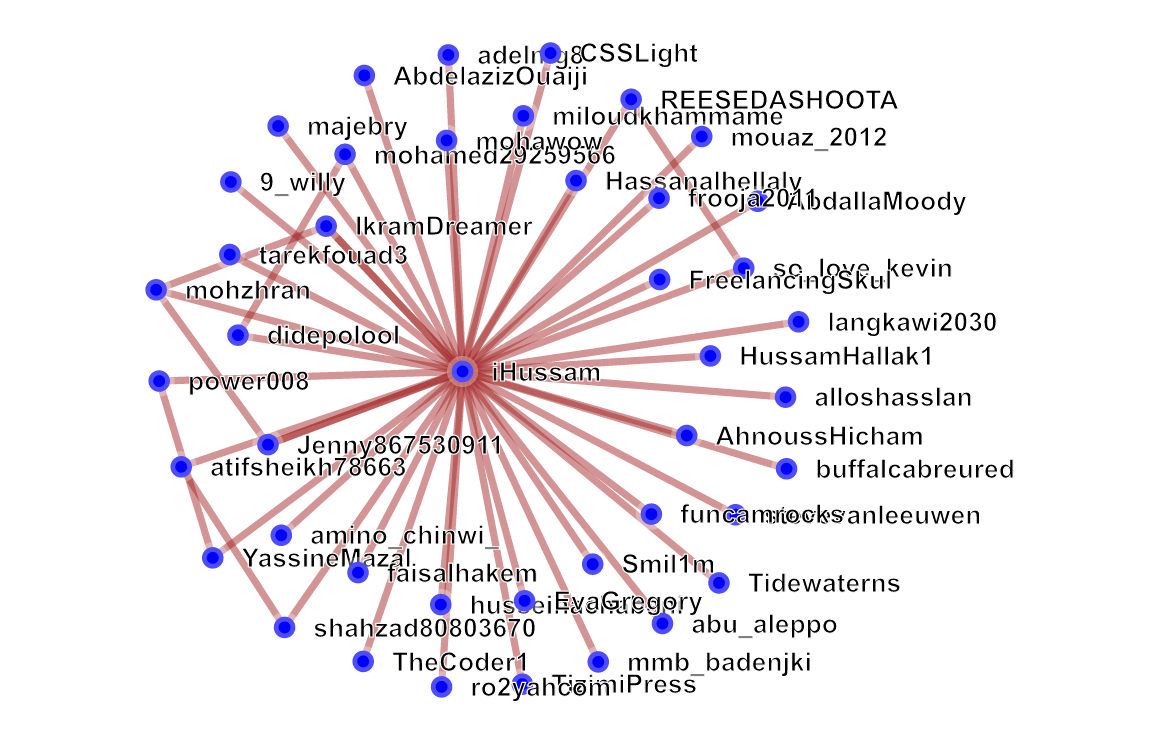
\includegraphics[scale=0.5]{d3.png}
\end{figure}


\subsection*{Included Files:}
config.py, getfollowers.py, iHussamFOLLOWERS.txt, whofollowswho.py, nodes.csv, links.csv, index.html, d3.png

\end{document}
